%----------------------------------------------------------------------------
%----------------------------------------------------------------------------
%				    	SETUP
%----------------------------------------------------------------------------
%----------------------------------------------------------------------------

\documentclass[11pt]{article}

%----------------------------------------------------------------------------
%			  	   PACKAGES
%----------------------------------------------------------------------------

%%%%%%%%%%%%%%%%%%%%%%%
% 	  Packages
%%%%%%%%%%%%%%%%%%%%%%%

%% Fonts and Symbols
%% --------------------------
\usepackage{
	amsmath,			% math operators
	amssymb,			% math symbols
	courier,			% better tt font for listings
  physics,      % provides \dv and \pdv for derivative happiness
	soul,				  % strike through with \st{}
	url,				 % embed urls in text
	xcolor,				% color!
}

% preserve default font for URLs
\renewcommand*{\UrlFont}{\rmfamily}		

%% Graphics
%% --------------------
\usepackage{
	graphicx,			% allows insertion of images
	subfigure,		% allows subfigures (a), (b), etc.
}				
\graphicspath{ {graphics/} }	% (graphicx) relative path to graphics folder				

%% Tables
%% --------------------------
\usepackage{
	booktabs,			% better tables, discourages vertical rulings
	multicol,			% allow multi columns
}

%% Layout Alteration
%% --------------------------
\usepackage{			
%	caption,			% line breaks in captions with \\
	geometry,			% change the margins for specific PAGES
	parskip,			% disable indents
	rotating,			% sideways figures
	setspace,			% single, double spacing
}
\geometry{			% specify page size options for (geometry)
	a4paper, 			% paper size
	hmargin=1in,	% horizontal margins
	vmargin=1in,	% vertical margins
}	


%% Units
%% --------------------------
\usepackage{
	siunitx,			% has S (decimal align) column type
}
\sisetup{input-symbols = {()},  % do not treat "(" and ")" in any special way
	group-digits  = false, 	% no grouping of digits
%	load-configurations = abbreviations,
%	per-mode = symbol,
}

%% Misc
%% --------------------------
\usepackage{
	enumitem,			% better control of enumerations, descriptions, etc
  todonotes,    % helpful todos in the doc
}

%% References
%% --------------------------
\usepackage[backend=biber,style=ieee]{biblatex}
\addbibresource{ELEC360_Lab_01.bib}

%----------------------------------------------------------------------------
%		     MACROS AND COMMANDS
%----------------------------------------------------------------------------

% override S column type with centered text column
\newcommand{\textcol}[1]{\multicolumn{1}{c}{#1}}


%----------------------------------------------------------------------------
%----------------------------------------------------------------------------
%				   DOCUMENT
%----------------------------------------------------------------------------
%----------------------------------------------------------------------------

\begin{document}

\doublespacing
\begin{titlepage}

\begin{center}
	\begin{LARGE}
		Department of Electrical and Computer Engineering \\
		University of Victoria \\
		ELEC 360 - Control Systems I \\[1cm]
		\textsc{Laboratory Report}
		\\[1cm]
	\end{LARGE}
\end{center}

\begin{tabular}{ p{0.25\textwidth} p{0.75\textwidth} }
	Experiment No.: & 0 \\ 
	Title: & Template \\ 
	Date of experiment:& 4 October, 2016 \\ 
	& \\
	Report submitted on:& 11 October, 2016 \\ 
	To: & Amirhosein Khazenifard, B04 \\ 
	& \\
  Lab Group No.: & 44 \\
	Names: & A.-K. Blanken (V00809798)\\
	& T. Stephen (V00812021) \\
  & S. Todesco (V00821678)
\end{tabular}

\end{titlepage}

\section{Summary}\label{sec:summary}
This experiment uses a Lab-Volt 5250 robotic arm (see Figure ~\ref{fig:arm}) to demonstrate the differences between angular, linear and GUI control modes.
\begin{figure}[tbph]
  \centering
  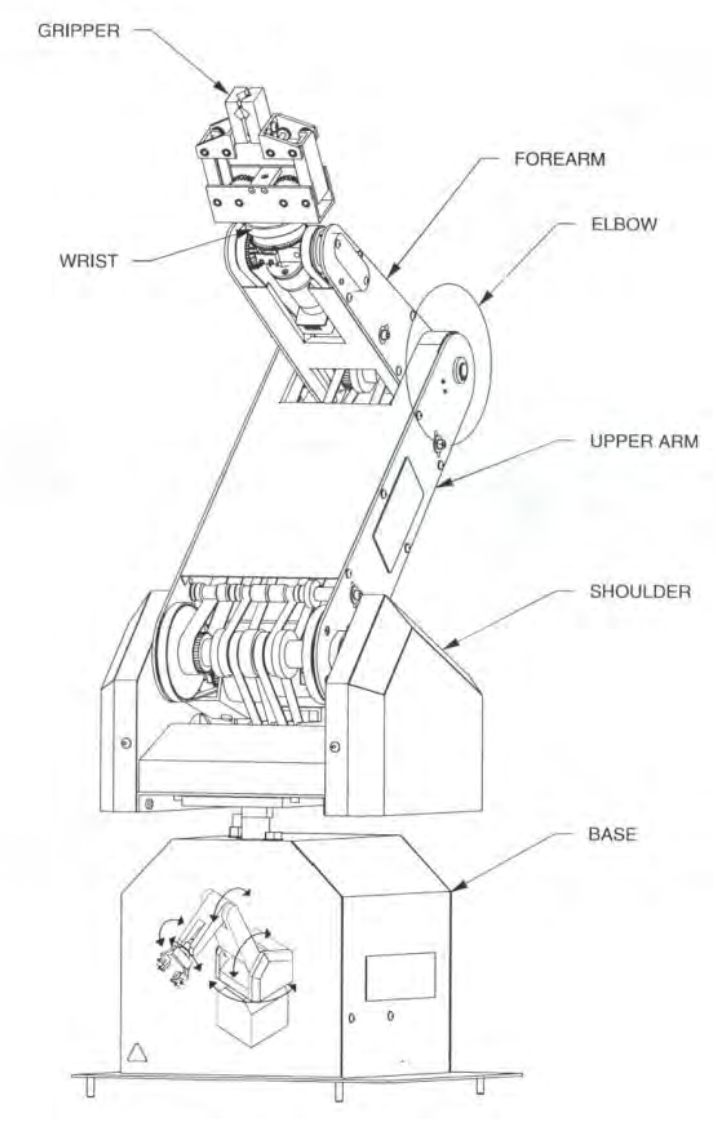
\includegraphics[width=0.4\linewidth]{graphics/arm}
  \caption{Lab-Volt 5250 robotic arm}
  \label{fig:arm}
\end{figure}

Angular and GUI modes allow the user to control the position of each robot joint.
Linear mode moves the tip of the robot's gripper through a Cartesian plane and determines the specific joint movements needed to achieve this motion.

\section{Introduction}\label{sec:intro}
The robot arm moved a stack of three blocks into the pyramid configuration shown in Figure~\ref{fig:blocks}.

\begin{figure}[tbph]
  \centering
  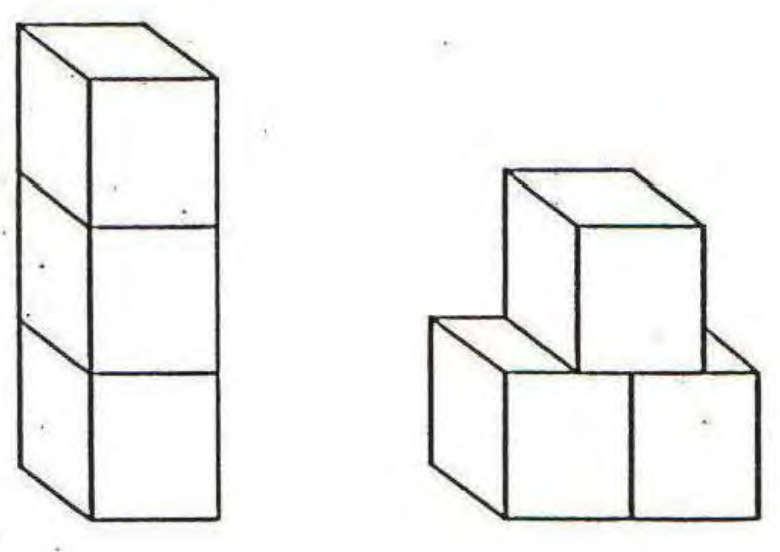
\includegraphics[width=0.4\linewidth]{graphics/blocks}
  \caption{Starting (left) and final (right) block configurations}
  \label{fig:blocks}
\end{figure}

This task was completed three times, each using a different command input method.
Starting at a known, fixed position (i.e. the \textit{hard home} of the arm), the arm is moved through space to move each block.
Critical points in the movement are marked as \textit{points} in the program.
When the program is played it runs through the entire sequence of points to move the blocks into the pyramid configuration.

The \textit{angular} input method allows each joint to be controlled independently.
Points can be created between successive joint movements but may also be combined.
The robot will execute all joint movements in parallel to transition between points.

The \textit{linear} input method allows the user to specify series of \textit{x, y, z} coordinates for the tip of the arm and the program will translate the $(x_i, y_i, z_i) \rightarrow (x_{i+1}, y_{i+1}, z_{i+1})$ spatial transition into the necessary joint movements.

Both angular and linear modes are controlled through the attached handheld controller (see Figure~\ref{fig:handheld}).

\begin{figure}[tbph]
  \centering
  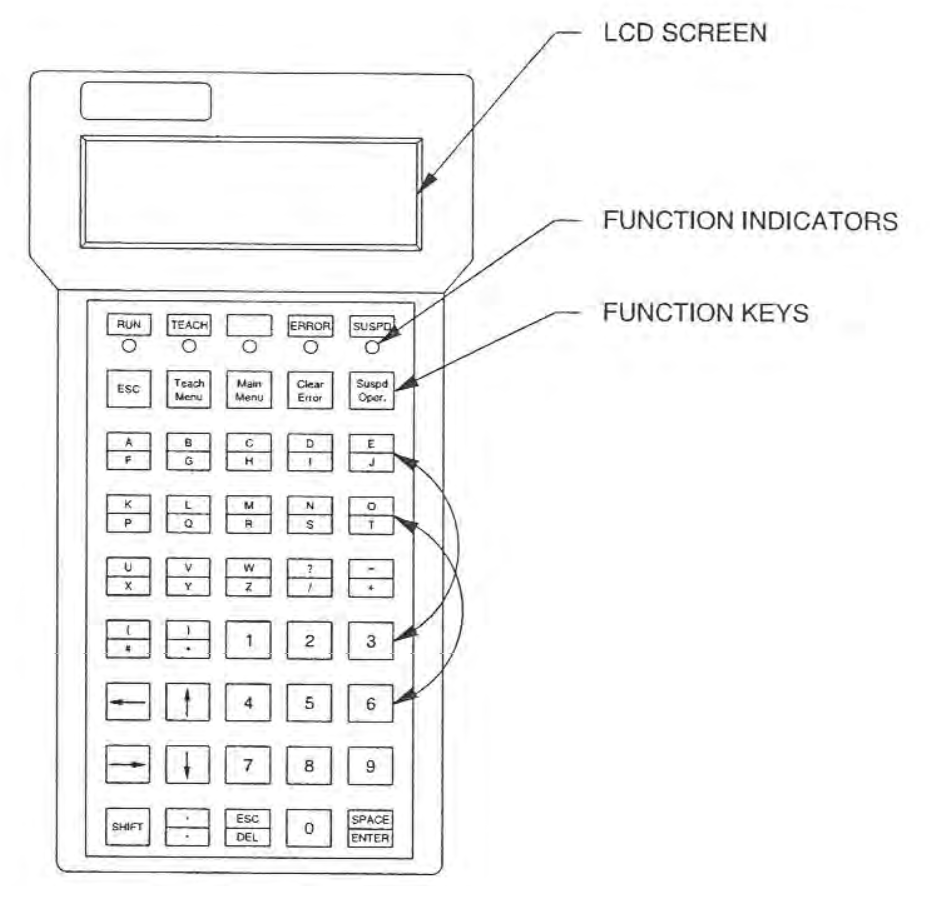
\includegraphics[width=0.4\linewidth]{graphics/handheld}
  \caption{Handheld controller for Lab-Volt 5250}
  \label{fig:handheld}
\end{figure}


\textit{GUI mode} records a sequence of joint measurements, identical to angular mode.
The GUI (see Figure~\ref{fig:gui}) provides the same functionality as the handheld controller but presents a history of the stored points on the right hand side.

\begin{figure}[tbph]
  \centering
  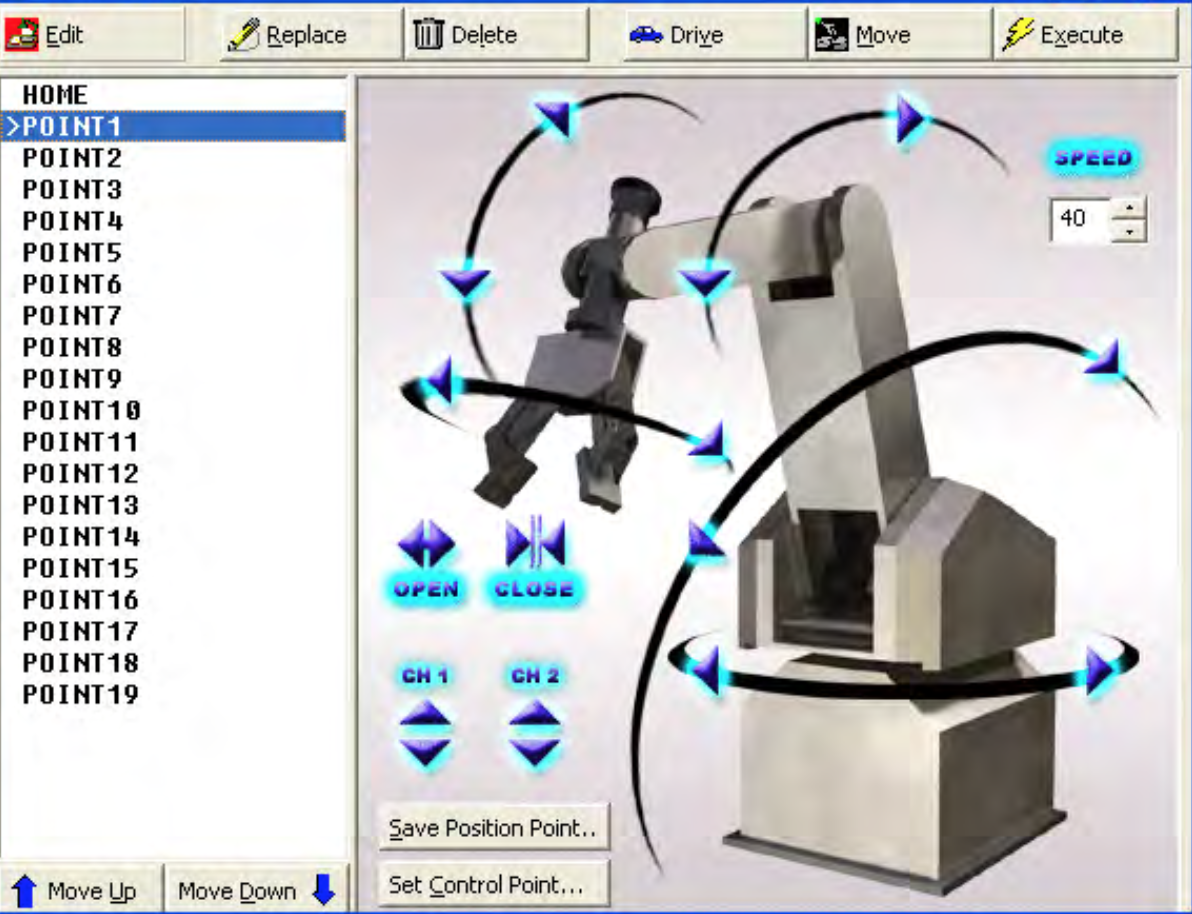
\includegraphics[width=0.4\linewidth]{graphics/gui}
  \caption{GUI for entering angular movement commands}
  \label{fig:gui}
\end{figure}


\input{sections/prelab}
\section{Results and discussion}\label{sec:results}
Sections \ref{sec:initial}, \ref{sec:mres}, and \ref{sec:mtorque} use static conditions to determine physical properties of the DC motor and parameters of its associated transfer function.
Section \ref{sec:bump} uses measured system input and output under dynamic conditions to determine the transfer function parameters.
The parameters derived from the prelab, static conditions and dynamic conditions are compared in Section \ref{sec:validation}.

\subsection{Initial experimental tests}\label{sec:initial}
The motor described in the lab manual \cite{lab-manual} is meant to be roughly equivalent to the motor used in the experiment.
One notable difference is that the lab manual motor has a maximum $u_m$ of \SI{15}{\volt} DC.
The QICii software used to control the experiment motor only allows a maximum $u_m$ of \SI{5}{\volt} DC.
To establish the validity of the lab manual motor parameters as approximations for the experiment motor we will compare the $\omega_{m\>max}$ from each source.

Using KVL in Figure~\ref{fig:motorschematic}, we can derive the relationship between the input voltage and the motor angular velocity as
\begin{equation}\label{eq:KVL}
  u_m(t) = R_m i_m(t) + L_m \pdv{i_m(t)}{t} + k_m \omega_m.
\end{equation}
Since $i_m(t) \approx \SI{0}{\ampere}$ at steady state, \eqref{eq:KVL} can be simplified and evaluated with the parameters from the manual
\begin{equation*}
  \omega_{m\>max} = {u_{m\>max} \over k_m} = {\SI{15}{\volt} \over \SI{0.0502}{\volt\second\per\radian}} = \SI{298.8}{\radian\per\second}.
\end{equation*}
For the experiment motor, $\omega_{m\>max}$ can be obtained directly from the QICii software.
The response for $u_{m\>max} = \SI{5}{\volt}$ is shown in Figure~\ref{fig:wmax}.
\begin{figure}[t!]
  \centering
  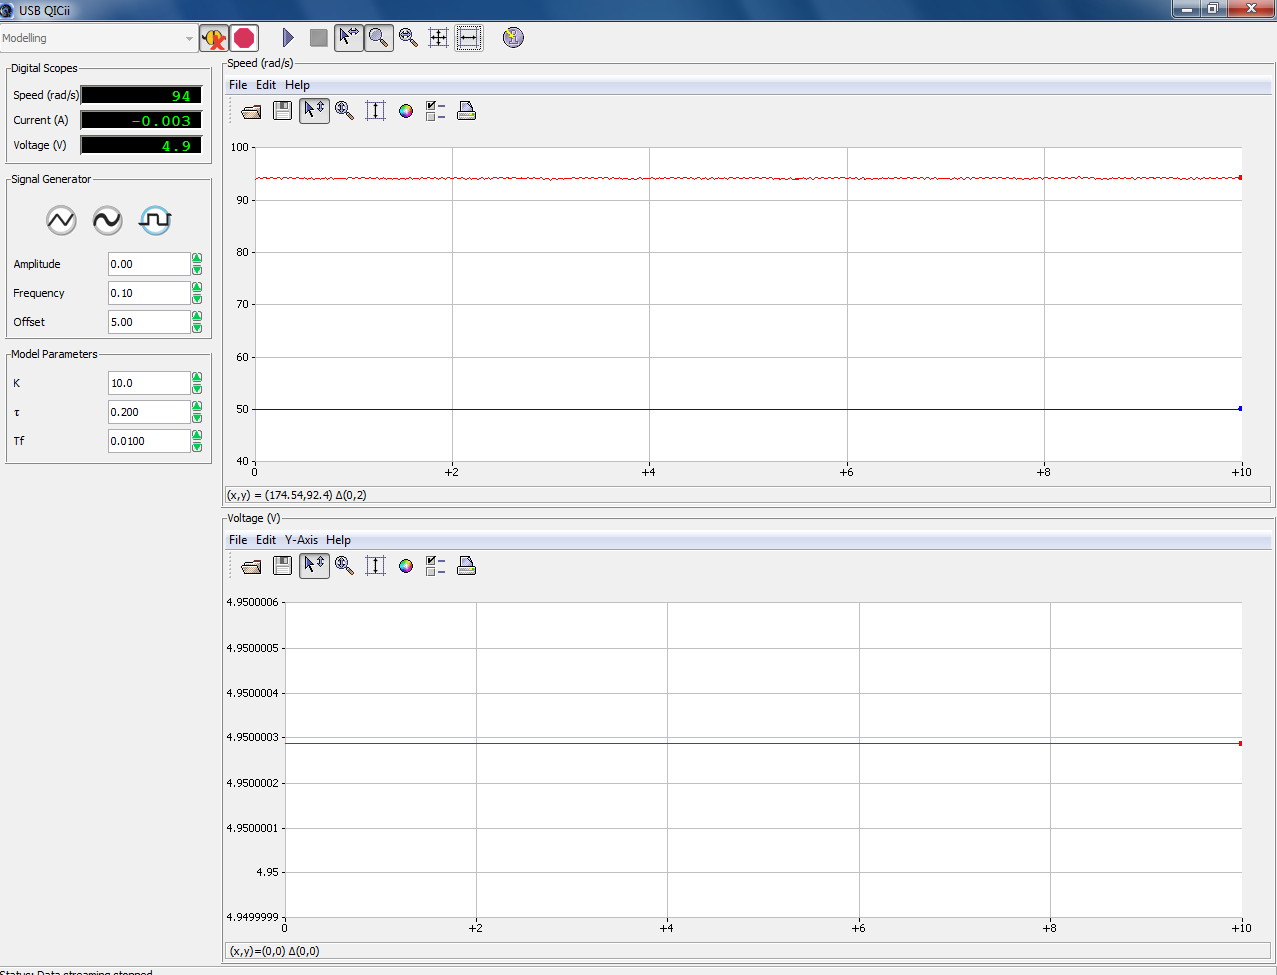
\includegraphics[width=0.95\linewidth]{graphics/part2}
  \caption{Steady state response of DC motor to constant $u_m$}
  \label{fig:wmax}
\end{figure}

\pagebreak
For the experiment motor
\begin{equation*}
  k_m = {\SI{4.95}{\volt} \over \SI{94}{\radian\per\second}} = \SI{0.05266}{\volt\second\per\radian}
\end{equation*}
which is slightly larger than the $k_m$ in the lab manual.
Thus, the physical parameters in the lab manual are valid.
The difference between the two sets of parameters will be explored in Section~\ref{sec:validation}.

\subsection{Motor resistance}\label{sec:mres}
If $\omega_m = 0$ in \eqref{eq:KVL} then we can determine $R_m$ by measuring $i_m$.
This constraint is realized by holding the disc stationary while applying different $u_m$.
Note, a bias current, $i_{m\>bias} = \SI{-10}{\milli\ampere}$ was measured when $u_m = \SI{0}{\volt}$.
The $R_m$ in each case is derived from \eqref{eq:KVL} as
\begin{equation*}
  R_m = {u_m \over i_m - i_{m\>bias}}
\end{equation*}
Table~\ref{table:Rm} summarizes these results.
\begin{table}[htpb]
  \centering
  \caption{Motor voltage and current at steady state}
  \label{table:Rm}
  \begin{tabular}{@{}SSS@{}}
    \toprule
      \multicolumn{1}{c}{$u_m$ (\si{\volt})} &
      \multicolumn{1}{c}{$i_m$ (\si{\ampere})} &
      \multicolumn{1}{c}{$R_m$ (\si{\ohm})} \\
    \midrule
    -5.00 & -0.35 & 14.3 \\
    -2.00 & -0.15 & 13.3 \\
     1.00 &  0.05 & 20.0 \\
     2.00 &  0.13 & 15.4 \\
     5.00 &  0.33 & 15.2 \\
    \bottomrule
      \multicolumn{2}{r}{$R_{m\>avg}$} & 15.6 \\
  \end{tabular}
\end{table}

The $R_{m\>avg}$ is nearly 50\% larger than the value of \SI{10.6}{\ohm} used for calculations in the prelab.
The source of this error can be seen in Figure~\ref{fig:motorschematic}.
$R_m$ is modeled as a lumped component but it represents the distributed resistance in the wires \textit{and} the motor.
The motor will experience a non-linear Coulomb friction at low voltages which this model lumps in to $R_m$.
The non-linear nature of the $R_m$ manifests as a spike at \SI{1}{\volt}.
Thus, the assumption that $R_m$ is constant and the motor is frictionless cause an underestimation in the prelab values.

\subsection{Motor torque constant}\label{sec:mtorque}
Similar to the approach in Section~\ref{sec:mres}, we can determine $k_m$ by analyzing the oppopsite static condition of the motor.
When the motor is in a steady state of motion, $i_m \approx 0$.
Using \eqref{eq:KVL}, we can determine
\begin{equation*}
  k_m = {u_m \over \omega_m}.
\end{equation*}
Table~\ref{table:km} summarizes the results, with $u_m$ varied over the same range as Section~\ref{sec:mres}.
\begin{table}[htpb]
  \centering
  \caption{Motor angular velocity in a free-spinning motor}
  \label{table:km}
  \begin{tabular}{@{}SSS@{}}
    \toprule
      \multicolumn{1}{c}{$u_m$ (\si{\volt})} &
      \multicolumn{1}{c}{$\omega_m$ (\si{\radian\per\second})} &
      \multicolumn{1}{c}{$k_m$ (\si{\volt\second\per\radian})} \\
    \midrule
    -5.00 & -93 & 0.0538 \\
    -2.00 & -35 & 0.0571 \\
    1.00 & 16 & 0.0625 \\
    2.00 & 35 & 0.0571 \\
    5.00 & 92 & 0.0543 \\
    \bottomrule
      \multicolumn{2}{r}{$k_{m\>avg}$} & 0.0570 \\
  \end{tabular}
\end{table}

This is larger than the prelab value of $k_m = \SI{0.0502}{\volt\second\per\radian}$.
This is because the prelab model underestimates $R_m$ and, since the motor does not perfectly conserve energy, $\omega_m$ will be slower than expected because of energy loss to friction and internal resistance.

\subsection{Open loop transfer function parameters from static analysis}\label{sec:tf-static}
Taking the Laplace transform of \eqref{eq:KVL} we can derive a first order transfer function of the form in \eqref{eq:tf}, where the open loop transfer function $G(s) = {\Omega_m(s) \over U_m(s)}$.
\begin{equation}\label{eq:KVL-tf}
  U_m(s) = R_m I_m(s) + s L_m I_m(s) + k_m \Omega_m(s)
\end{equation}
\cite{lab-manual} tells us that
\begin{equation*}
  J_{eq} \dot{\omega}_m(t) = k_m i_m(t) + T_d.
\end{equation*}
Disturbance torques can be neglected by ensuring the motor spins without interruption in the laboratory.
The previous equation can be written in the Laplace domain as
\begin{equation}\label{eq:tf-load}
  sJ_{eq} \Omega_m(s) = k_m I_m(s).
\end{equation}
Substituting \eqref{eq:tf-load} into \eqref{eq:KVL-tf} yeilds
\begin{equation*}
  {\Omega_m(s) \over U_m(s)} = {k_m \over L_m J_{eq}s^2 + R_m J_{eq} s + {k_m}^2}.
\end{equation*}
For a small motor $R_m \gg L_m$, so the effect of $L_m$ can be neglected in our linear model.
The previous equation can be rewritten as
\begin{equation*}
  {\Omega_m(s) \over U_m(s)} = { 1 \over k_m \left( {J_{eq} R_m \over {k_m}^2} s + 1 \right)}.
\end{equation*}
Comparing the previous equation with the form of \eqref{eq:tf} implies
\begin{equation}\label{eq:static-params}
  K = {1 \over k_m} \quad \text{and} \quad \tau = {J_{eq} R_m \over {k_m}^2}.
\end{equation}
\cite{lab-manual} gives values for $J_m$, $M_l$ and $R_l$ which can be used to determine $J_{eq}$.
\begin{align*}
  J_{eq} &= J_m + {1 \over 2} M_l {R_l}^2 \\
         &= \left(\SI{11.6}{\gram\square\centi\meter}\right) + {1 \over 2} \left(\SI{68}{\gram}\right) \left(\SI{2.48}{\centi\meter}\right)^2 \\
         &= \SI{220.7}{\gram\square\centi\meter} \\
         &= \SI{2.207e-5}{\kilogram\square\meter}
\end{align*}
$J_{eq}$, $k_{m\>avg}$ and $R_{m\>avg}$ can be substituted into \eqref{eq:static-params} to yeild $K = \SI{17.55}{\radian\per\volt\per\second}$ and $\tau = \SI{0.106}{\second}$.
The prelab has $K = \SI{19.92}{\radian\per\volt\per\second}$ and $\tau = \SI{0.093}{\second}$.
The smaller gain and larger time constant represent the losses in the system to internal resistance and friction as well as the effect of $L_m$ to inhibit motor acceleration.

\subsection{Bump test}\label{sec:bump}
$K$ and $\tau$ can also be derived by only measuring the input $u_m$ and output $\omega_m$ during the application of a step input.
This technique is referred to as a ``bump test.''
Assuming the measured system has a first order response, the output will be
\begin{equation}\label{eq:dynamic-yt}
  y(t) = \Delta u K \left(1 - e^{{-t \over \tau}}\right).
\end{equation}
$K$ will be the ratio of steady state output to input
\begin{equation}\label{eq:dynamic-gain}
  K = {\Delta y \over \Delta u}.
\end{equation}
Substituting \eqref{eq:dynamic-gain} into \eqref{eq:dynamic-yt} at $t = \tau$ gives
\begin{equation}\label{eq:dynamic-tau}
  y(\tau) = \Delta y \left(1 - e^{-1}\right) \approx 0.63 \Delta y.
\end{equation}
The step input $u_m$ will be approximated by a square wave varying between \SI{1}{\volt} and \SI{5}{\volt} ($\Delta u = \SI{4}{\volt}$) and a frequency of \SI{0.4}{\hertz}.
The period between edges is long enough so that the motor will achieve its steady state behavior.
Figure~\ref{fig:step} shows the response of the DC motor to this input.
\pagebreak
\begin{figure}[tbph]
  \centering
  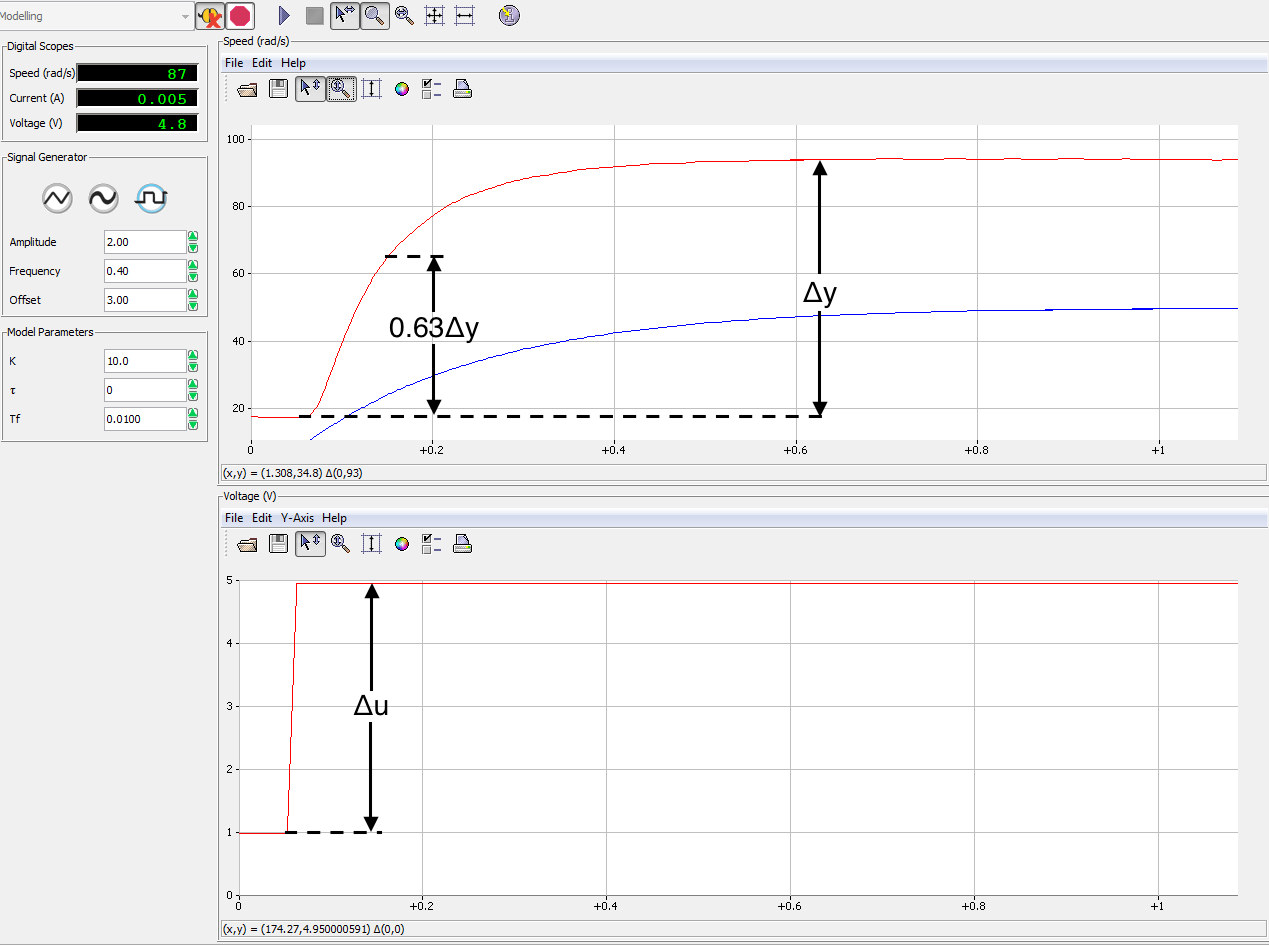
\includegraphics[width=0.95\linewidth]{graphics/part3}
  \caption{Response of DC motor to step input}
  \label{fig:step}
\end{figure}

The response of the motor is $\Delta y = \SI{75}{\radian\per\second}$.
It reaches $0.63 \Delta y$ at $\Delta t = \SI{0.091}{\second} = \tau$. \eqref{eq:dynamic-gain} gives $K = \SI{18.75}{\radian\per\volt\per\second}$.
These values are closer to the prelab values than those in Section~\ref{sec:tf-static}.

\subsection{Model validation}\label{sec:validation}
QUCii will take values of $K$ and $\tau$ and use them to generate an expected response to the measured input.
The square wave from Section~\ref{sec:bump} is reused as a step input.
Figure~\ref{fig:validation} shows models with parameters derived from the prelab, static analysis and bump test.
The model parameters in Figure~\ref{subfig:tuned} were determined be the best fit from manual parameter variation.
The expected response is in dark blue and the measured response is in red.
\begin{figure}[t!]
  \subfigure[Prelab: $K = \SI{19.92}{\radian\per\volt\per\second}$, $\tau = \SI{0.93}{\second}$]
  {
    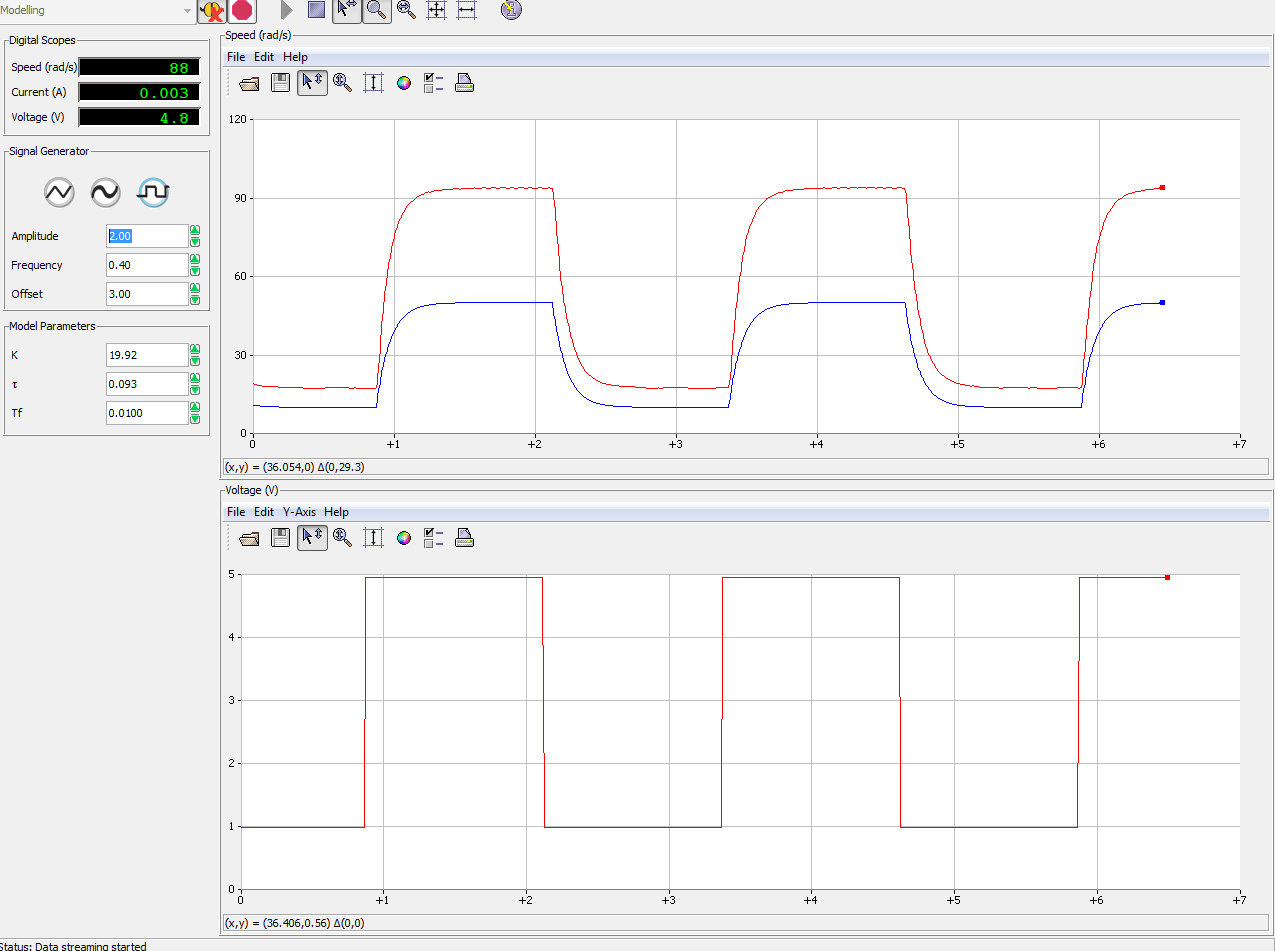
\includegraphics[width=0.475\linewidth]{part4_prelab}
    \label{subfig:prelab}
  }
  \subfigure[Static analysis: $K = \SI{17.5}{\radian\per\volt\per\second}$, $\tau = \SI{0.106}{\second}$]
  {
    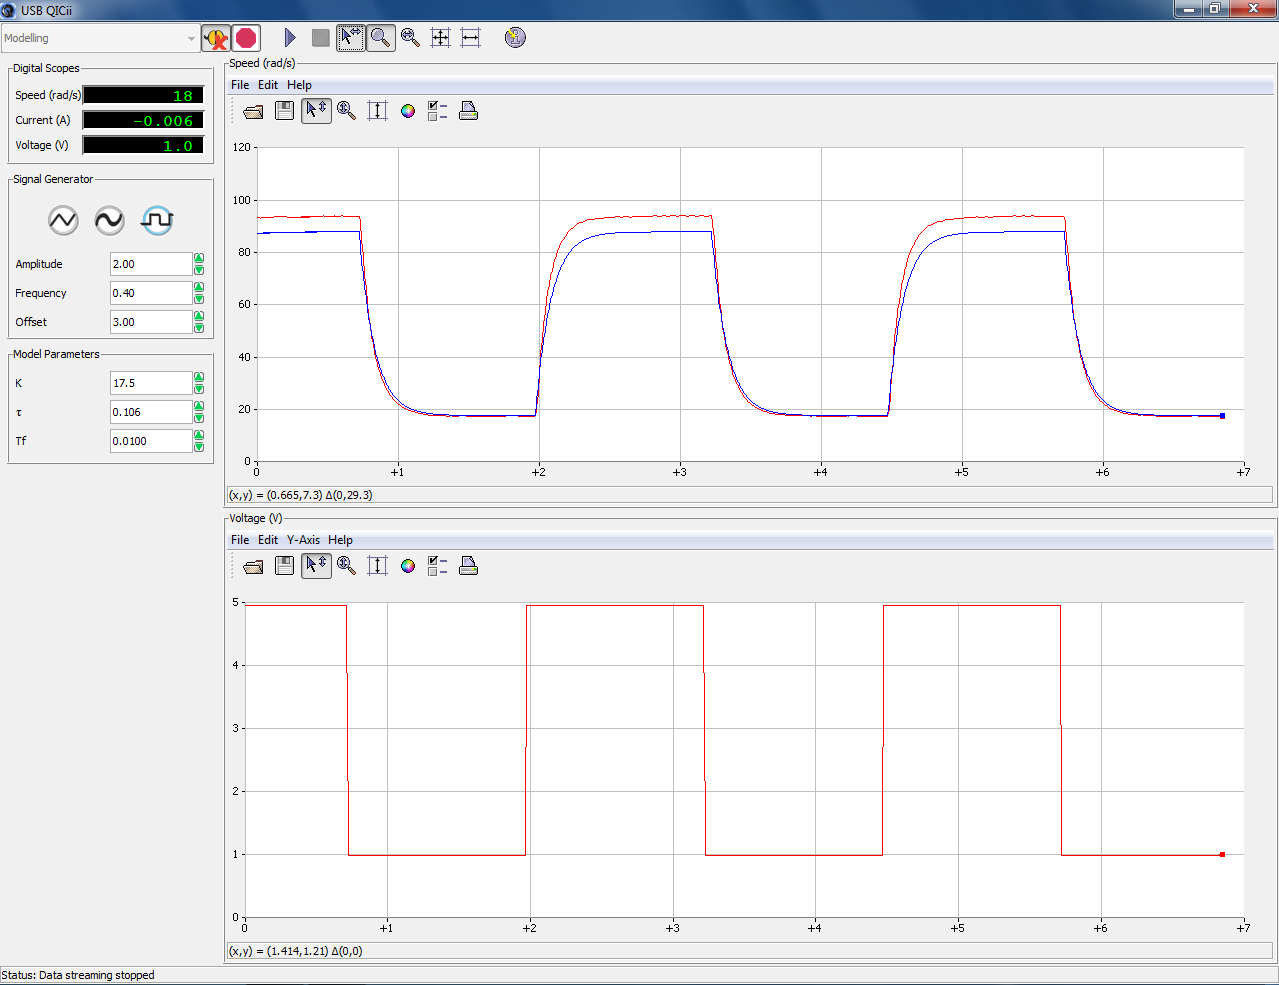
\includegraphics[width=0.475\linewidth]{part4_static}
    \label{subfig:static}
  }
  \subfigure[Bump test: $K = \SI{18.8}{\radian\per\volt\per\second}$, $\tau = \SI{0.091}{\second}$]
  {
    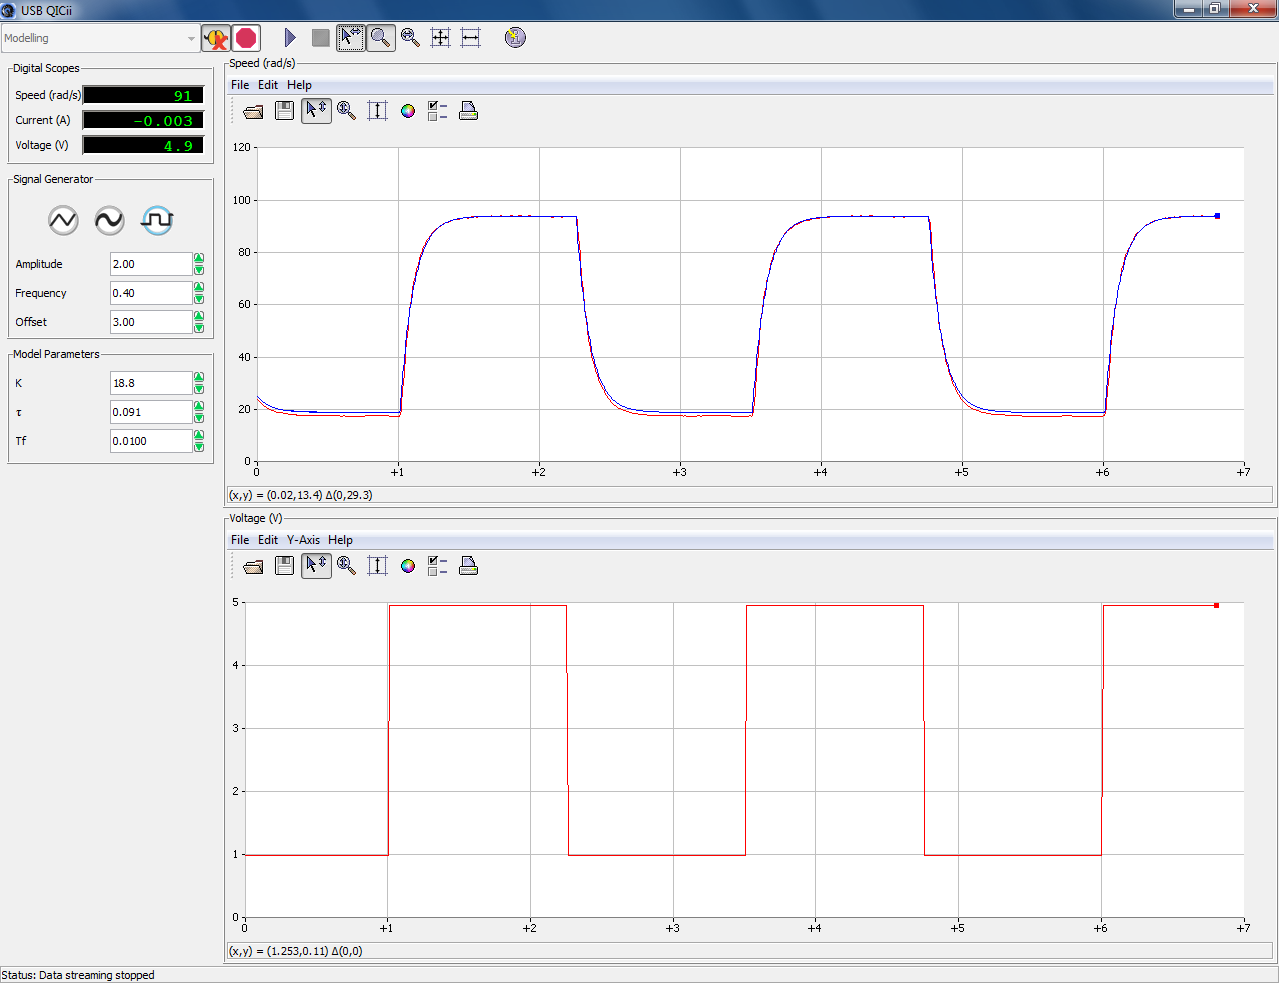
\includegraphics[width=0.475\linewidth]{part4_bump}
    \label{subfig:bump}
  }
  \subfigure[Tuned: $K = \SI{18.6}{\radian\per\volt\per\second}$, $\tau = \SI{0.090}{\second}$]
  {
    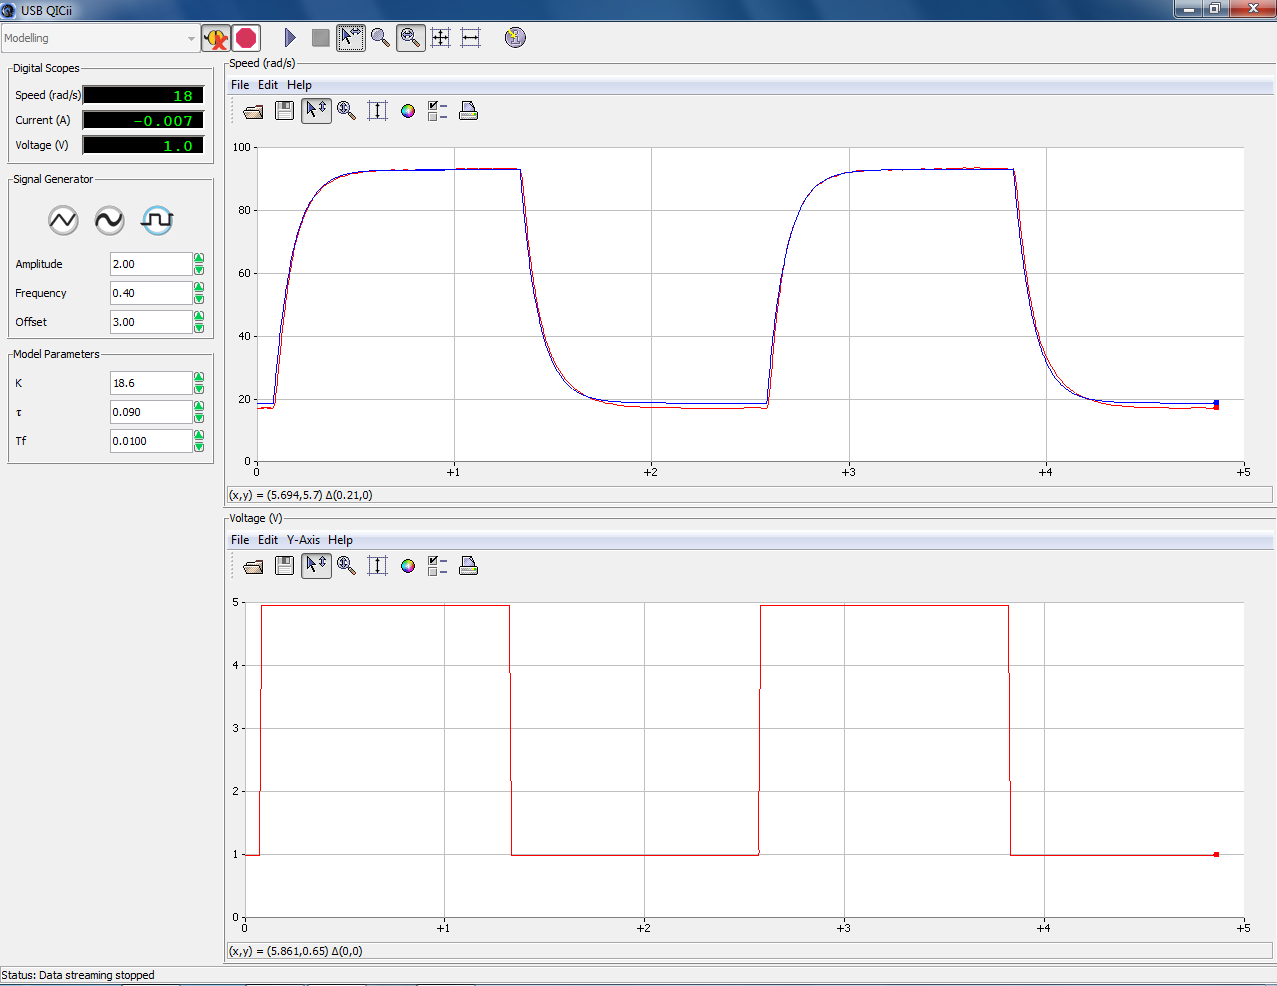
\includegraphics[width=0.475\linewidth]{part4_tuned}
    \label{subfig:tuned}
  }
  \caption{Performance of various models against measured motor response to step input}
  \label{fig:validation}
\end{figure}

The performance of the models is inversely correlated to the number of assumptions they make about the physical system at hand.
The prelab values of $R_m$ and $k_m$ did not precisely match those from Sections~\ref{sec:mres} and \ref{sec:mtorque} and its model is the furthest from the actual behavior of the motor.

The model derived from static analysis ignored the effects of $L_m$ and $T_d$ entirely and $i_m$ and $\omega_m$ when it was convenient.
The static analysis model performs considerably better than the prelab model but it underestimates the motor response at the upper steady state.

The bump test model performs extremely well.
It tracks the ``up'' response perfectly.
The model deviates very slightly on the ``down'' response, where it fails to track the observed decay of $\omega_m$ at steady state.
This deviance is likely due to a breakdown of the linear model as $u_m \rightarrow \SI{0.4}{\volt}$, the voltage at which the motor overcomes the Coulomb friction and begins to rotate.
Observe the spike in $R_m$ in Table~\ref{table:Rm} at $u_m = \SI{1.00}{\volt}$.
This suggests Coulomb friction is significant over a range of values and manifests as non-linear behavior at low voltages. 

The tuned model is not a significant improvement over the bump test model.
This is because the non-linearities from Coulomb friction cannot be accounted for by varying $K$ and $\tau$ in a linear model.

\section{Conclusion}\label{sec:conclusion}
Justify conclusions and results.


\printbibliography[heading=bibintoc,title={References}]

\end{document}
